In questo capitolo si procederà con un confronto dei punteggi di penalità ottenuti con le diverse strategie. Si noti che verranno riportati i punteggi di penalità, di volta in volta, relativi alla stessa mappa nelle stesse condizioni per ogni strategia. Ogni sezione è strutturata con la figura della mappa in questione, con eventualmente una breve descrizione a indicare perché la mappa possa essere interessante, e con il confronto tra le prestazioni delle varie strategie sulla mappa in questione.

\section{Mappa di default}
La prima mappa utilizzata è quella di default fornita nello scheletro del progetto, illustrata in figura \ref{fig:default-all}. È una mappa piuttosto regolare, che non presenta alcuna insidia particolare se non quella di avere, in basso a sinistra, una cella di tipo urban che, se visitata, porterebbe l'UAV a una posizione in cui l'uscita non sarebbe raggiungibile. Mediante il modulo \ref{sec:uscita}, presente in ogni strategia, tutte le tecniche usate evitano questo piccolo ostacolo. Ecco un elenco riassuntivo delle penalità:
\begin{enumerate}
	\item Strategia Safe (cap. \ref{cap:safe}): 36386
	\item Strategia di Base (cap. \ref{cap:base}): 42863
	\item Strategia con Punteggi Relativi (cap. \ref{cap:rel}): 45310
	\item Strategia Loiter Monitoring di Base (cap. \ref{cap:loiter-base}): 42538
	\item Strategia Loiter Monitoring con Punteggi Relativi (cap. \ref{cap:loiter-rel}): 46935
\end{enumerate}

La mappa non è molto significativa perché non enfatizza particolarmente nessun vantaggio di una strategia rispetto a un'altra. È chiaro però che la strategia Safe, per sua natura, cercando un massimo assoluto relativo a una sola cella, individua, tendenzialmente, zone meno interessanti da esplorare rispetto alle altre strategie (in effetti vengono prese in esame prima tutte le celle urban e, solo successivamente, le celle rural). Migliora notevolmente la situazione con la strategia di base, la quale dirigendosi verso "zone" interessanti più che verso "celle" interessanti, riesce a minimizzare il cammino da un estremo all'altro della mappa, risparmiando più tempo.
A causa di una sfortunata conformazione della mappa, risulta meno efficace la strategia con punteggi relativi. Quest'ultima dovrebbe ridurre ulteriormente il tragitto dell'UAV, ma si ritrova a lasciare per ultima, proprio perché poco interessante, la cella in basso a sinistra (che risulta poco "interessante" in quanto circondata da border, hills e lake), dovendo percorrere tutta la mappa trasversalmente per fare l'inform dell'ultima cella rimasta. Da notare che per tutte queste prime tre strategie il tempo su questa mappa è sufficiente a fare tutte le inform, quindi la penalità è solamente influenzata dal tempo rimanente.

\begin{figure}
        \centering
        \begin{subfigure}[b]{0.5\textwidth}
                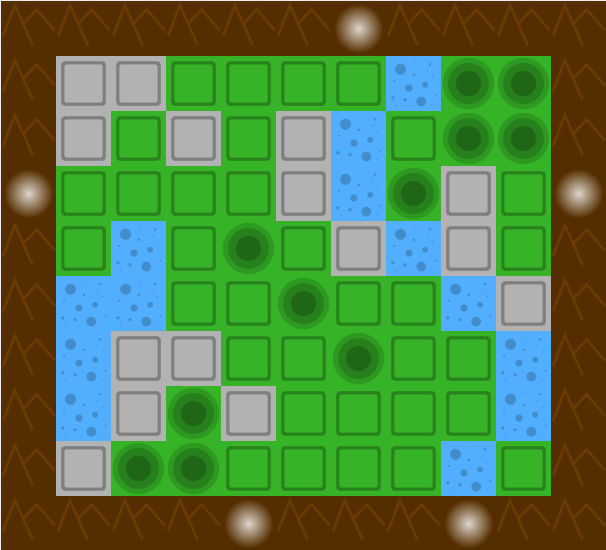
\includegraphics[width=\textwidth]{maps/default.png}
                \caption{Mappa pre-allagamento}
                \label{fig:default-pre}
        \end{subfigure}%

        \begin{subfigure}[b]{0.5\textwidth}
                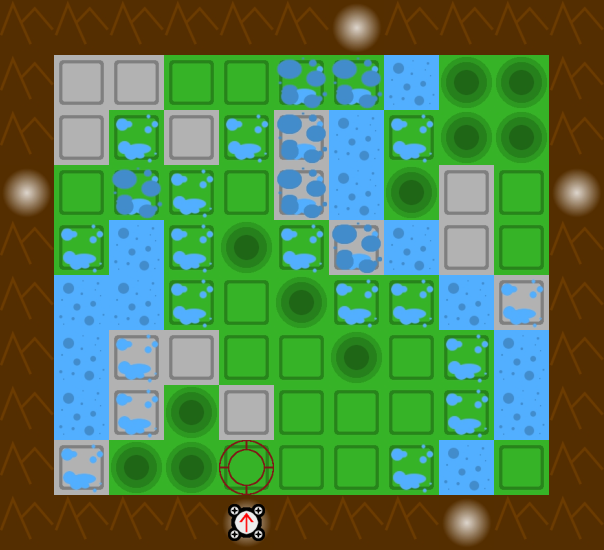
\includegraphics[width=\textwidth]{maps/default-flood.png}
                \caption{Mappa post-allagamento}
                \label{fig:default-post}
        \end{subfigure}
       
        \caption{Mappa di Default, Tempo a disposizione: 1000}\label{fig:default-all}
\end{figure}

\section{Altre mappe}

Abbiamo quindi testato il comportamento dell'UAV su altre cinque mappe: due scarsamente urbanizzate (di seguito "sparse"), una piccola ("S.p.") e una grande ("S.g."); due fittamente urbanizzate (di seguito "dense"), una piccola ("D.p.") e una grande ("D.g."); infine una che presenta molte "valli", ossia ha la caratteristica che alcuni punti vicini in linea d'aria sono in realtà molto distanti in quanto a cammino, poiché presentano molte celle di tipo "hill" da aggirare. Ecco una tabella riassuntiva:
\begin{center}
    \begin{tabular}{| p{4cm} | l | l | l | l | l |} \hline
                                    & \textbf{S.p.} & \textbf{D.p.} & \textbf{S.g.} & \textbf{D.g.} & \textbf{Valli}    \\ \hline
    Safe                            & 77983         & 158510        & 194659557     & 197414050     & 233762191         \\ \hline
    Base                            & 93248         & 268105        & 201783694     & 210322087     & 235693437         \\ \hline
    Punteggi Relativi               & 94657         & 154623        & 168806229     & 174043061     & 180090655         \\ \hline
    Loiter Base                     & 78878         & 4475479       & 194792541     & 217665525     & 233808312         \\ \hline
    Loiter con Punteggi Relativi    & 81199         & 179787        & 168806229     & 177287886     & 180090655         \\ \hline
    \end{tabular}
\end{center}
